% ------------------------------------------------------------------------------
% TYPO3 Version 10 LTS - What's New (English Version)
%
% @author	Michael Schams <schams.net>
% @license	Creative Commons BY-NC-SA 3.0
% @link		https://typo3.org/help/documentation/whats-new/
% @language	English
% ------------------------------------------------------------------------------

\section{Dashboard}
\begin{frame}[fragile]
	\frametitle{Dashboard}

	\begin{center}\huge{\color{typo3darkgrey}\textbf{Dashboard}}\end{center}
	\begin{center}\large{\textit{System information, news, and much more for backend users}}\end{center}

\end{frame}

% ------------------------------------------------------------------------------
% Feature | 90333 | Dashboard

\begin{frame}[fragile]
	\frametitle{Dashboard}
	\framesubtitle{Backend View}

	A dashboard has been introduced that shows important system information to the currently logged-in backend user.

	\begin{figure}
		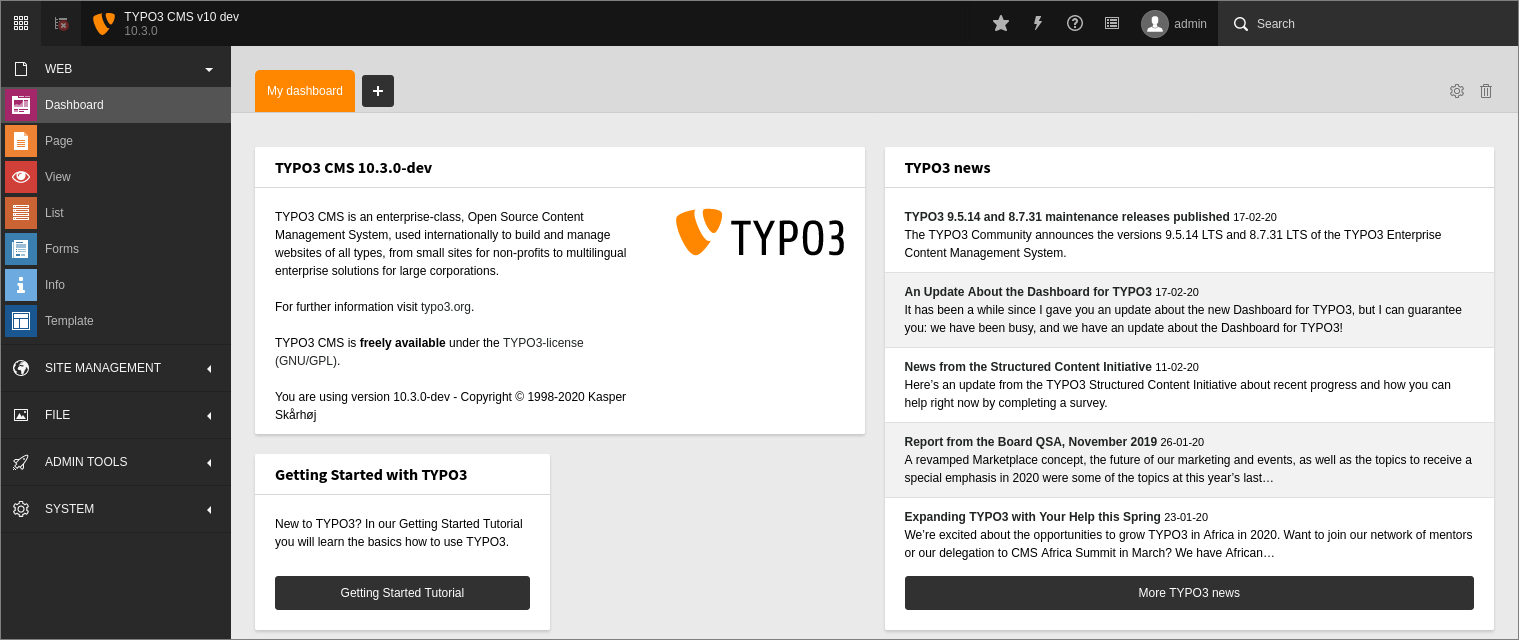
\includegraphics[width=0.9\linewidth]{Dashboard/90333a-Dashboard.png}
	\end{figure}

\end{frame}

% ------------------------------------------------------------------------------
% Feature | 90333 | Dashboard

\begin{frame}[fragile]
	\frametitle{Dashboard}
	\framesubtitle{Backend View}

	Users can create their own dashboards and add, remove, and re-arrange "widgets".

	\begin{figure}
		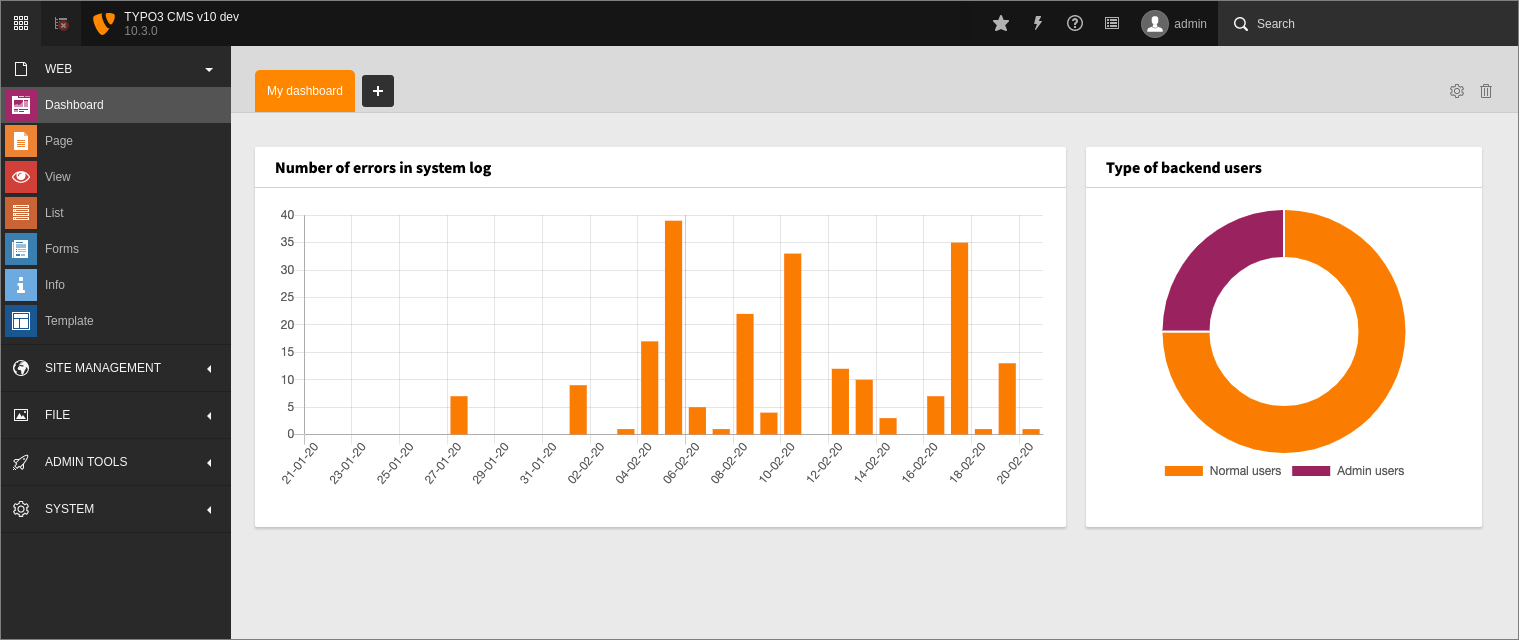
\includegraphics[width=0.9\linewidth]{Dashboard/90333b-Dashboard.png}
	\end{figure}

\end{frame}

% ------------------------------------------------------------------------------
% Feature | 90333 | Dashboard

\begin{frame}[fragile]
	\frametitle{Dashboard}
	\framesubtitle{Options for Integrators}

	% decrease font size for code listing
	\lstset{basicstyle=\tiny\ttfamily}

	\begin{itemize}
		\item Dashboard \textit{presets} can be configured for new users or for users who deleted all their dashboards.
		\item This can be used to show a "Getting Started" dashboard by default.
		\item Example TSconfig:

\vspace{-0.4cm}
\begin{lstlisting}
options.dashboard.dashboardPresetsForNewUsers = default, dashboardPreset-myPreset
\end{lstlisting}

		\item Multiple dashboard presets can be defined in a comma separated list.
	\end{itemize}

\end{frame}

% ------------------------------------------------------------------------------
% Feature | 90333 | Dashboard

\begin{frame}[fragile]
	\frametitle{Dashboard}
	\framesubtitle{Custom Widgets}

	\begin{itemize}
		\item TYPO3 v10 LTS comes with a number of widgets out of the box\newline
			\smaller
				(for example: general information, failed backend logins, TYPO3 news, links to the documentation, etc.)
			\normalsize
		\item Developers can easily build custom widgets as extensions.
		\item Register and configure widgets in a YAML file:\newline
			\small
				\texttt{EXT:myextension/Configuration/Services.yaml}
			\normalsize
		\item The "Dashboard" system extension provides some typical widgets types\newline
			\smaller
				(bar chart, call-to-action button, doughnut chart, list, number with icon, and rss widget)
			\normalsize
		\item Read more about the dashboard in the
			\href{https://docs.typo3.org/c/typo3/cms-dashboard/master/en-us/}{TYPO3 documentation}.

	\end{itemize}

\end{frame}

% ------------------------------------------------------------------------------
